% ----------------------------------------------------
% Methodology
% ----------------------------------------------------

\chapter{Salinometer Evaluation and Testing}\label{ch:testing}

\section{Overview}

Several tests were conducted to evaluate the salinometer.
The tests experimentally verified the accuracy of the individual components, evaluated the salinometer's interaction with saltwater samples and determined its ability and accuracy in measuring salinity.
The tests were conducted in two phases because some required access to the board's circuitry and test points, while others required the probe to be exposed to salt water, which could only happen after the probe was cast in epoxy.
The first phase involved evaluating the \gls{dac}, \gls{adc}, calibration resistor and resistance measuring accuracy which is covered in \refsec{sec:dac-voltage-range-and-accuracy} to \refsec{sec:resistance-measuring-accuracy}.

After the first testing phase, the probe was cast into epoxy resin as described in \refsec{sec:probe-epoxy-casting}, which allowed the second phase to commence.
The second phase involved establishing a voltage-resistance relationship for the salt water, a voltage-to-conductivity relationship for both electrodes and finally, the salinometer's ability to measure salinity, which is covered in \refsec{sec:linear-conductivity-measurement} to \refsec{sec:salinity-measurement-accuracy}.
A summary of these tests is shown in \reftbl{tab:testing-summary}, and each test is discussed in further detail in their relevant sections.

%chktex-file 44
\begin{longtblr}[
    caption = {A summary of the evaluation and testing of the salinometer.},
    label = {tab:testing-summary}
    ]{
    hlines,
    vlines,
    colspec = {Q[c,m,1cm]X[c,m]*{3}{Q[c,m,1.75cm]}}
    }
    \textbf{Sec.} & \textbf{Test Description} & \textbf{Result Metric} & \textbf{Ideal Result} & \textbf{Measured Results} \\
    \ref{sec:dac-voltage-range-and-accuracy} & The minimum and maximum voltage output of the \gls{dac} between $0V$ and $V_{DD} = 3,3V$ & Range & $0-3,3V$ & $0-2,59V$ \\
    \ref{sec:dac-voltage-range-and-accuracy} & The gain and offset of the output voltage of the \gls{dac} relative to the instructed voltage & {Gain \\ Offset} & {$1,0$ \\ $0,0V$} & {$0,9837$ \\ $0,0070V$} \\
    \ref{sec:adc-accuracy} & The gain and offset of the voltage measured by the \gls{adc} relative to the voltage measured by the multimeter & {Gain \\ Offset} & {$1,0$ \\ $0,0V$} & {$0,9877$ \\ $0,0082V$} \\
    \ref{sec:calibration-resistance} & The resistance of the calibration resistor $R_{CAL}$ & Resistance & $5\Omega$ & $5,00\Omega$ \\
    \ref{sec:resistance-measuring-accuracy} & The gain and offset of the resistance measured by the salinometer relative to the resistance measured by the multimeter & {Gain \\ Offset} & {$1$ \\ $0\Omega$} & {$1,0000$ \\ $0,0000\Omega$} \\
\end{longtblr}

\section{Testing Apparatus}

Voltage and resistance measurements were taken on the probe using a bench multimeter.
The most accurate multimeter available was a \textit{Keysight Technologies} U3401A, shown in \reffig{fig:bench-multimeter}, which had voltage accuracy of $0,02\%$ and resistance accuracy of $0,1\%$.
In order to test the probe \gls{pcb}, voltage probes were connected to the test points, shown in \reffig{fig:probe-experiments}, or they were connected directly to the components.

\begin{figure}[ht]
    \begin{minipage}{0.5\textwidth}
        \centering
        \includegraphics[width=0.7\textwidth]{Figures/probe_experiments}
        \caption{The salinometer probe with multimeter cables attached to a test point and ground.}
        \label{fig:probe-experiments} %chktex 24
    \end{minipage}
    \begin{minipage}{0.5\textwidth}
        \centering
        \includegraphics[width=\textwidth]{Figures/bench_multimeter}
        \caption{The bench multimeter used for the tests displaying a voltage reading.}
        \label{fig:bench-multimeter} %chktex 24
    \end{minipage}
\end{figure}

\section{DAC Voltage Range and Accuracy}\label{sec:dac-voltage-range-and-accuracy}

The transistor buffer configuration explained in \refsec{sec:dac-voltage-range-and-accuracy} has one disadvantage: the output voltage of the system is limited by the transistor's $V_{BE}$ where the highest possible voltage output is $V_{DD} - V_{BE}$.
According to the transistor's \href{https://www.lcsc.com/datasheet/lcsc_datasheet_2310131500_Jiangsu-Changjing-Electronics-Technology-Co---Ltd--S8050-J3Y-RANGE-200-350_C2146.pdf}{data sheet}, the buffered output should be limited to $3,3V - 0,6V = 2,7V$ when conducting $0A$ and $3,3V - 0,75V = 2,55V$ when conducting the circuit's maximum current of $33mA$.
In order to assess the range and accuracy of the \gls{dac}, it was instructed to output voltages from $0V$ to $V_{DD} = 3,3V$ in intervals of 64-bit. 
The output voltage was measured at the base and emitter of the transistor, with no load and a maximum load of $100\Omega$.
The results were graphed and shown in~\reffig{fig:dac-voltage-range-no-load} and~\reffig{fig:dac-voltage-range-loaded}.

\begin{figure}[ht]
    \centering
    \begin{minipage}{.5\textwidth}
        \centering
        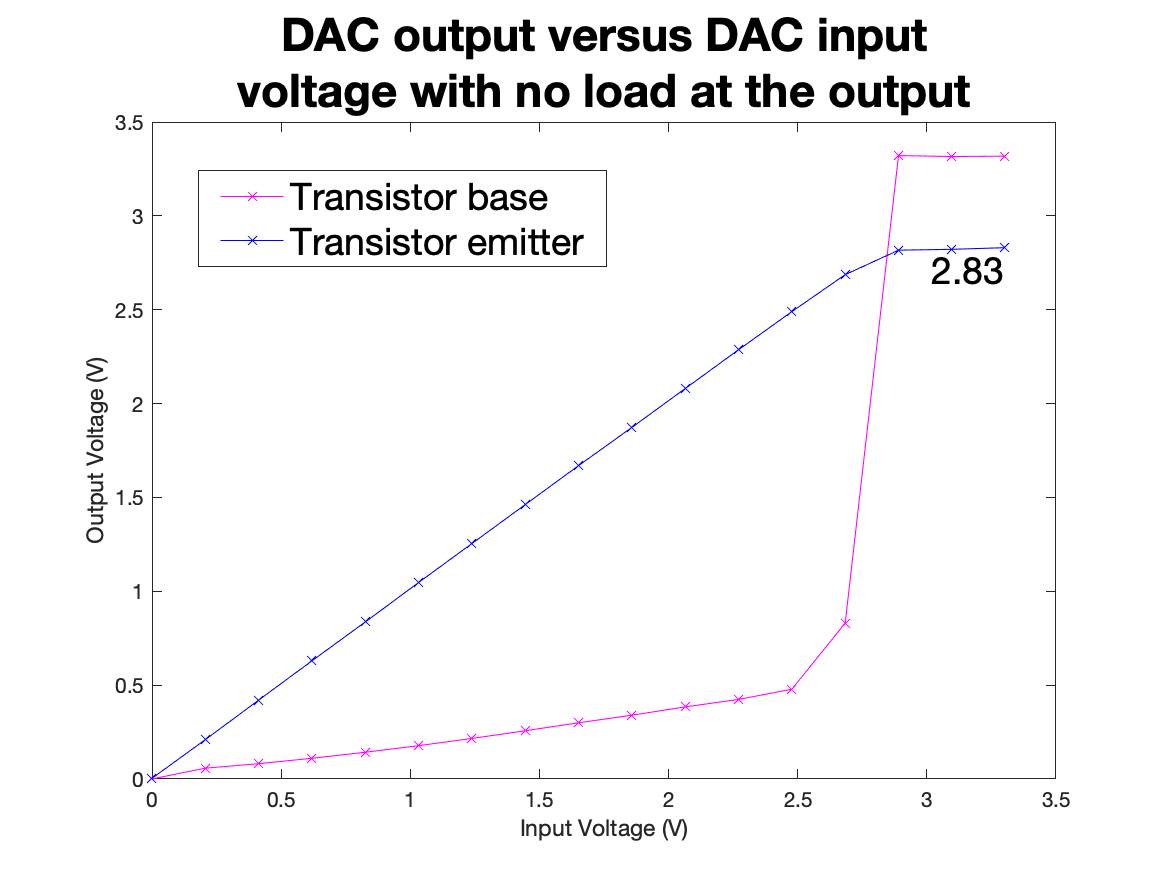
\includegraphics[width=\textwidth]{Figures/Testing/DAC_no_load}
        \caption{The input voltage versus the output voltage of the \gls{dac} with no load.}
        \label{fig:dac-voltage-range-no-load} %chktex 24
    \end{minipage}%
    \begin{minipage}{.5\textwidth}
        \centering
        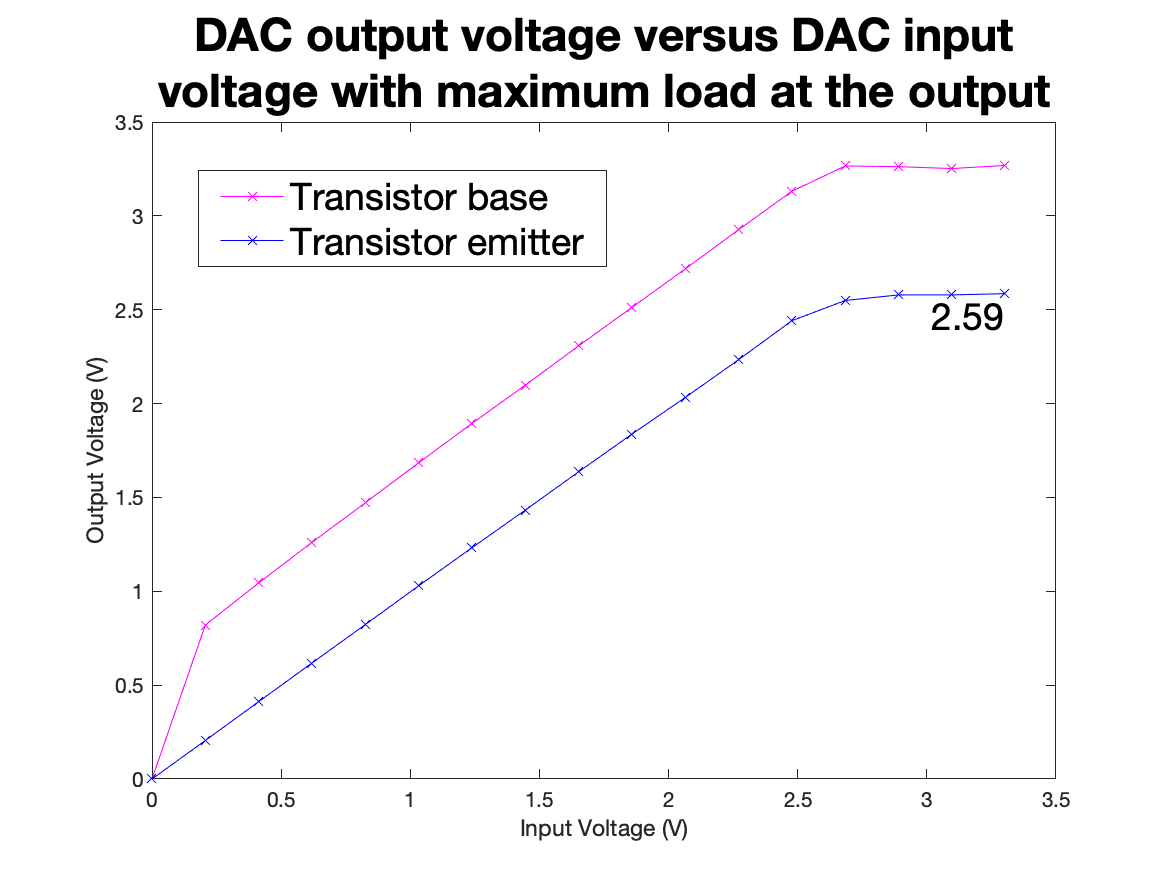
\includegraphics[width=\textwidth]{Figures/Testing/DAC_loaded}
        \caption{The input voltage versus the output voltage of the \gls{dac} with the maximum load of $100\Omega$.}
        \label{fig:dac-voltage-range-loaded} %chktex 24
    \end{minipage}
\end{figure}

The voltage drop due to $V_{BE}$ can clearly be seen on~\reffig{fig:dac-voltage-range-loaded}.
The unloaded output voltage reached $2,83V$, and the loaded output voltage reached $2,59V$, which were slightly higher than the predicted limits.

An alternative attempt was made to achieve a higher voltage output using the \gls{dac}'s internal voltage reference of $1,21V$ multiplied by a gain of $4$, resulting in a reference of $4,84V$.
As expected, this did not increase the output voltage; the base of the transistor continued to measure $3,3V$ and the emitter $2,83V$ while unloaded.

Due to the voltage limitations, the \gls{dac} was limited to $2,6V$ for future testing and implementation.
When excluding the voltage readings above $2,6V$, the \gls{dac} achieved a gain of $0,9837V/V$ and an offset $+0,0070V$ between the input voltage and measured voltage under maximum load. 
\section{ADC Accuracy}\label{sec:adc-accuracy}

The \gls{adc} was tested by measuring a range of voltages produced by the \gls{dac} and comparing them to the multimeter's measurement.
The \gls{adc} was configured in 12-bit mode, with each measurement taking 15 \gls{adc} clock cycles, equivalent to $250ns$ with the $16MHz$ system clock.
$5$ measurements were taken and averaged for each voltage outputted by the \gls{dac} to increase the accuracy of each measurement.
The results were graphed and shown in~\reffig{fig:adc-accuracy}. 

\begin{figure}[ht]
    \centering
    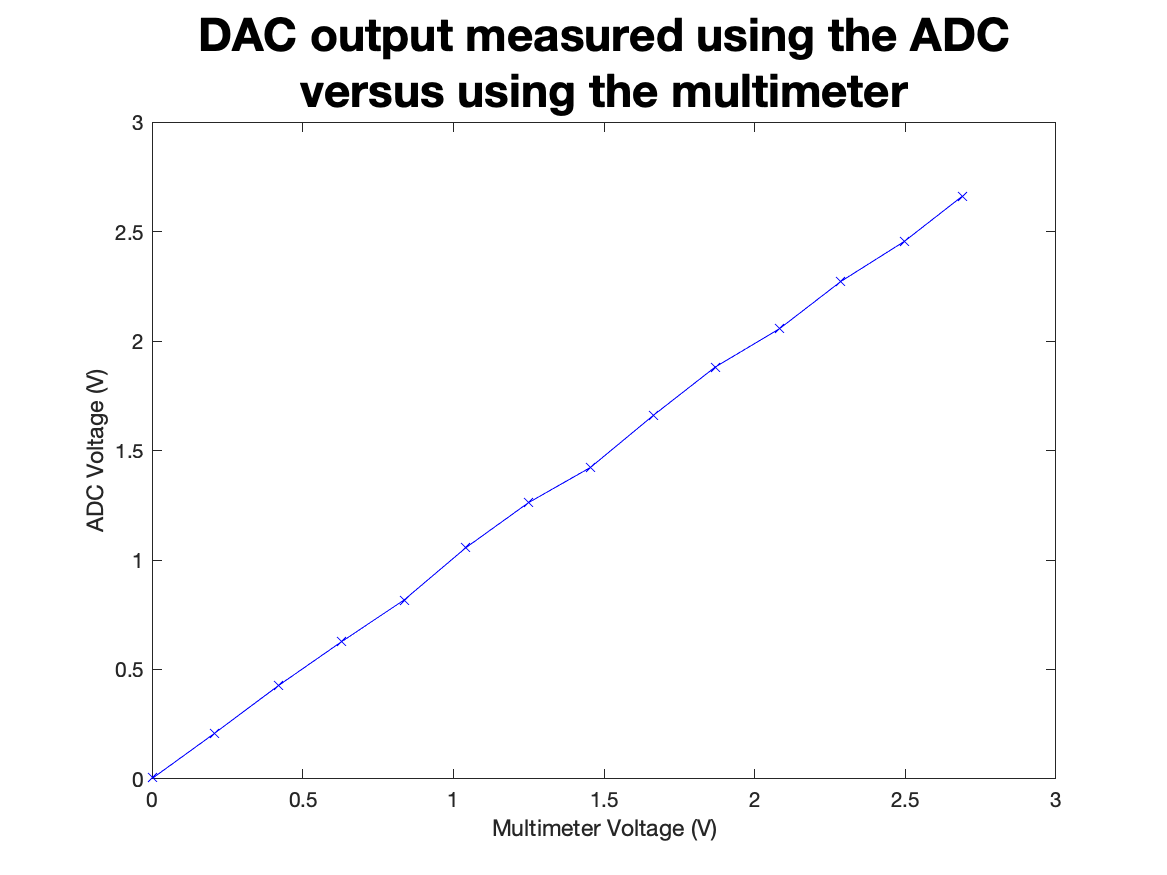
\includegraphics[width=0.5\textwidth]{Figures/Testing/ADC}
    \caption{The voltage output by the \gls{dac} measured by a multimeter versus by the \gls{adc}.}
    \label{fig:adc-accuracy} %chktex 24
\end{figure}

The \gls{adc} achieved a gain of $0,9877V/V$ and an offset of $0,0082V$ compared to the multimeter.

\section{Calibration Resistance}\label{sec:calibration-resistance}

The multimeter measured the calibration resistor by directly connecting its probes to the four parallel resistors.
The calibration resistor was electrically disconnected from the rest of the circuit during the measurement.
The calibration resistance was specified to be $5\Omega \pm 0,25\%$; thus, its actual value could range between $4,9875$ and $5,0125\Omega$.

The multimeter measured the calibration resistor to be $5,25\Omega$.
However, the multimeter probes measured $0,25\Omega$ when short-circuited.
Thus, the actual resistance was calculated as $5,00\Omega$.
It should be noted that the multimeter can only display to the nearest $0,01\Omega$.
Thus, the actual resistance could range from $4,995\Omega$ to $5,005\Omega$, and more precise equipment would be required to obtain a more accurate measurement.

\section{Resistance Measuring Accuracy}\label{sec:resistance-measuring-accuracy}

The probe's accuracy in measuring resistance was determined by comparing its calculated resistance to the multimeter's measurement of a given resistor.
The probe calculated resistance by measuring the voltage drop across the resistor attached between the titanium electrode ports and the calibration resistor. 
Then, it calculated its resistance per \refeqn{eqn:parallel-resistor-total} to \refeqn{eqn:parallel-resistor-uncertainty}.

For this test, the probe measured resistance using two methods: one with a single voltage provided by the \gls{dac} of $V_{DD}/2 = 1,65V$ and one with voltage sweep from the \gls{dac} with $50$ samples.
In the latter case, the resistances were calculated for each sample and averaged.
At low voltages, single-bit errors caused significant changes in the calculated resistance, which were avoided by limiting the voltage sweep to between $0,3V$ and $2,6V$.
The resistors used had a range of $0\Omega$, or a short-circuit, to $10\Omega$ as this is the expected range for the gold electrodes.
The results of the voltage sweep versus the multimeter test are shown in~\reffig{fig:resistance-measuring-accuracy-uncorrected}. 

\begin{figure}[!ht]
    \centering
    \begin{minipage}{.5\textwidth}
        \centering
        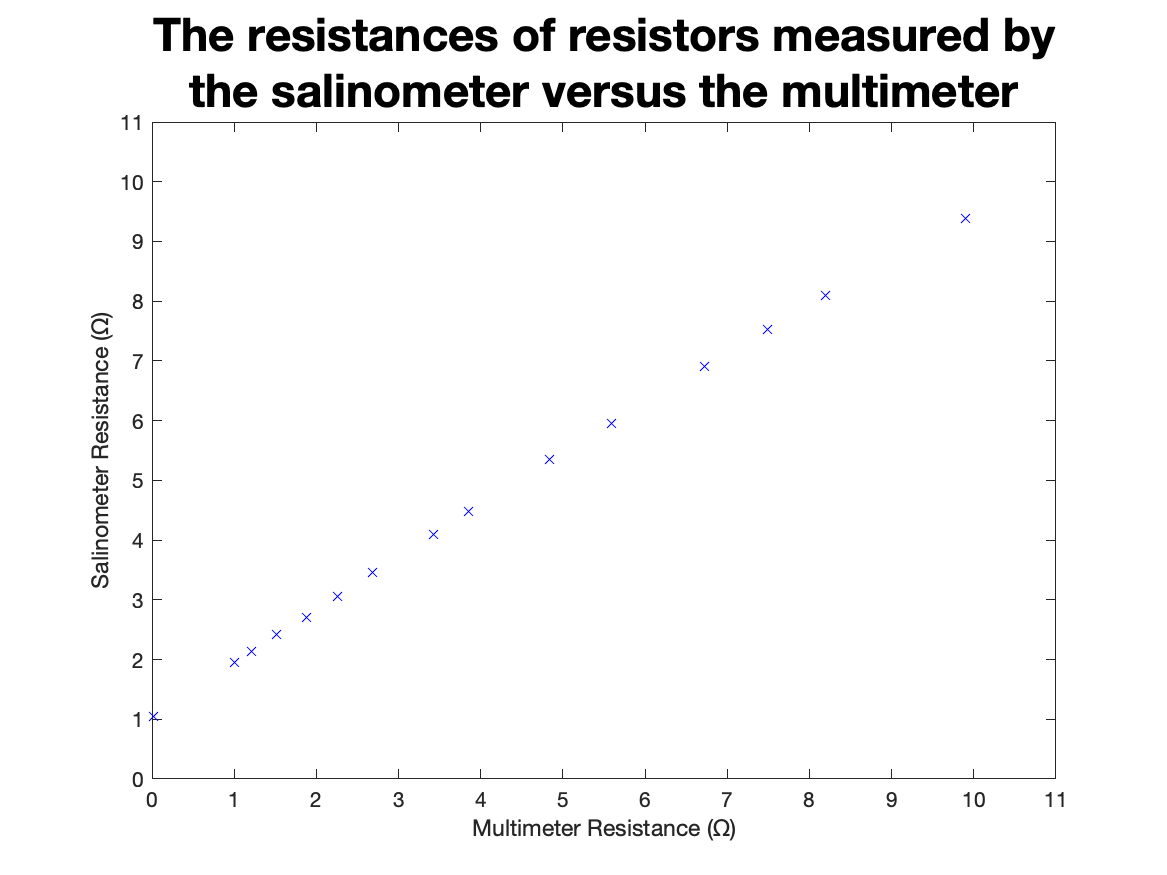
\includegraphics[width=\textwidth]{Figures/Testing/R_uncorrected}
        \caption{The resistance measuring test.}
        \label{fig:resistance-measuring-accuracy-uncorrected} %chktex 24
    \end{minipage}%
    \begin{minipage}{.5\textwidth}
        \centering
        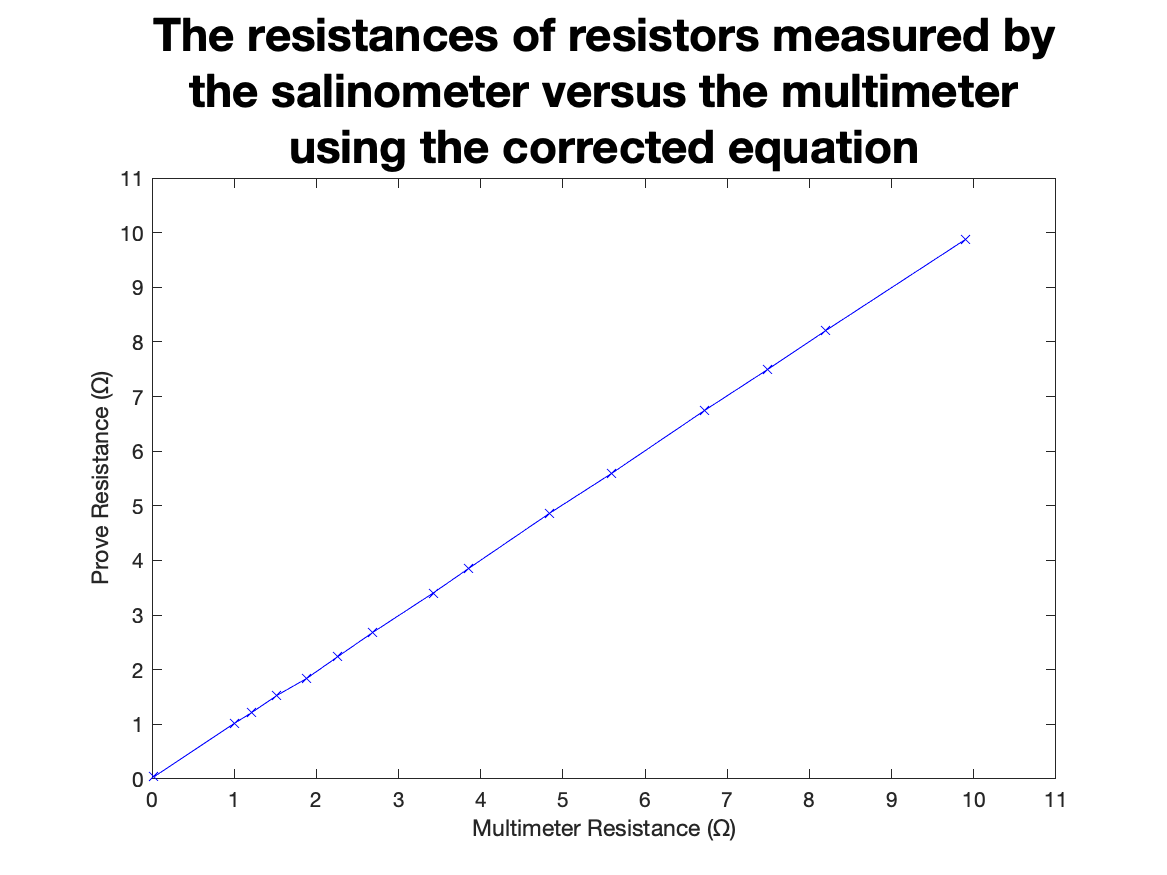
\includegraphics[width=\textwidth]{Figures/Testing/R_corrected}
        \caption{The resistance measuring test using the corrected equation.}
        \label{fig:resistance-measuring-accuracy-corrected} %chktex 24
    \end{minipage}
\end{figure}

The single voltage and voltage sweep methods were perfectly correlated with an $r^2$ value of $1,0000$.
However, there was a clear error between the probe's and the multimeter's measurements.
This error was assumed to be due to the unaccounted resistance of the switches and the traces.
While these values could be measured and included in the equation, a more efficient and arguably more accurate method would be to generate an equation of best fit and use it to calculate the correct resistance.


To determine the general formula of the equation of best fit, \refeqn{eqn:electrode-calib-resistance} was adjusted to include $r_e$, which represents the unknown resistance of the switches and traces as shown in \refeqn{eqn:resistance-measuring}.
The $R_{calibration}$, $R_1$ and $r_e$ were condensed into the standard rational function coefficients $p$ and $q$ as shown in \refeqn{eqn:resistance-rational}.
Finally, the equation was rearranged to give the electrode's resistance in terms of the measured voltage ratio as shown in \refeqn{eqn:resistance-measuring-rational}.

\begin{align}
 V_{ratio} &= \lfrac{\lfrac{R_{electrode} + r_{e1}}{R_{electrode} + R_1 + r_{e2}}}{\lfrac{R_{calibration} + r_{e3}}{R_{calibration} + R_1 + r_{e4}}} \nonumber \\
    &= \lfrac{R_{electrode} + r_{e1}}{R_{electrode} + R_1 + r_{e2}} \times \lfrac{R_{calibration} + R_1 + r_{e4}}{R_{calibration} + r_{e3}} \label{eqn:resistance-measuring} \\
 V_{ratio} &= \lfrac{p_1 R_{electrode} + p_2}{R_{electrode} + q_1} \label{eqn:resistance-measuring-rational} \\
 R_{electrode} &= \lfrac{p_2 - q_1 V_{ratio}}{V_{ratio} - p_1} \label{eqn:resistance-measuring-rearranged}
\end{align}

The \refeqn{eqn:resistance-measuring-rational} of best fit was confirmed using MATLAB, which gave the values $p_1 = 17,4687$, $p_2 = 18,4643$ and $q_1 = 91,8315$ with an $r^2$ value of $1,0000$. 
The corrected resistance values were obtained from the previous data set by reversing the previous formula and applying \refeqn{eqn:resistance-measuring-rearranged} to the voltage ratios.
These results were graphed and are shown in \reffig{fig:resistance-measuring-accuracy-corrected} and have a gain of $1,0000$ and an offset of $0,0000$.
Note that this correction equation is only valid when $R_1$ is $100\Omega$ and separate equations will need to be generated should different values of $R_1$ be needed.

\section{Voltage Sweep Repeatability}\label{sec:voltage-sweep-repeatability}

The following tests investigate a method for producing repeatable voltage measurements of a saltwater sample.
In order to conduct these tests, the probe was cast into epoxy as described in \refsec{sec:probe-epoxy-casting}.

The tests were configured with parameters such as which electrodes to use, the voltage sample count, the \gls{adc} sample count and the \gls{dac} range.
Due to a circuit error discovered after the epoxy casting, the gold electrodes could only be used with the fringe guard.
Thus, the effectiveness of the fringe guard was unable to be tested.
Each voltage sweep produced the specified number of samples, which were transmitted over \gls{uart} to a computer, where they were processed using Microsoft Excel and MATLAB to generate graphs and metrics.

The first test was a simple voltage sweep performed both forwards and in reverse with increasing and decreasing \gls{dac} voltages, respectively.
The test was configured with the gold electrodes and the fringe guard, 50 voltage samples, 2 \gls{adc} samples and a voltage range of $0-2,6V$.
It was performed on a salt water sample of unknown salinity around 30 on the Practical Salinity Scale PSS-78.
Ideally, the two sweeps should have been identical.
However, they were not, as shown in \reffig{fig:test1}.

\begin{figure}[ht]
    \begin{minipage}{0.5\textwidth}
        \centering
        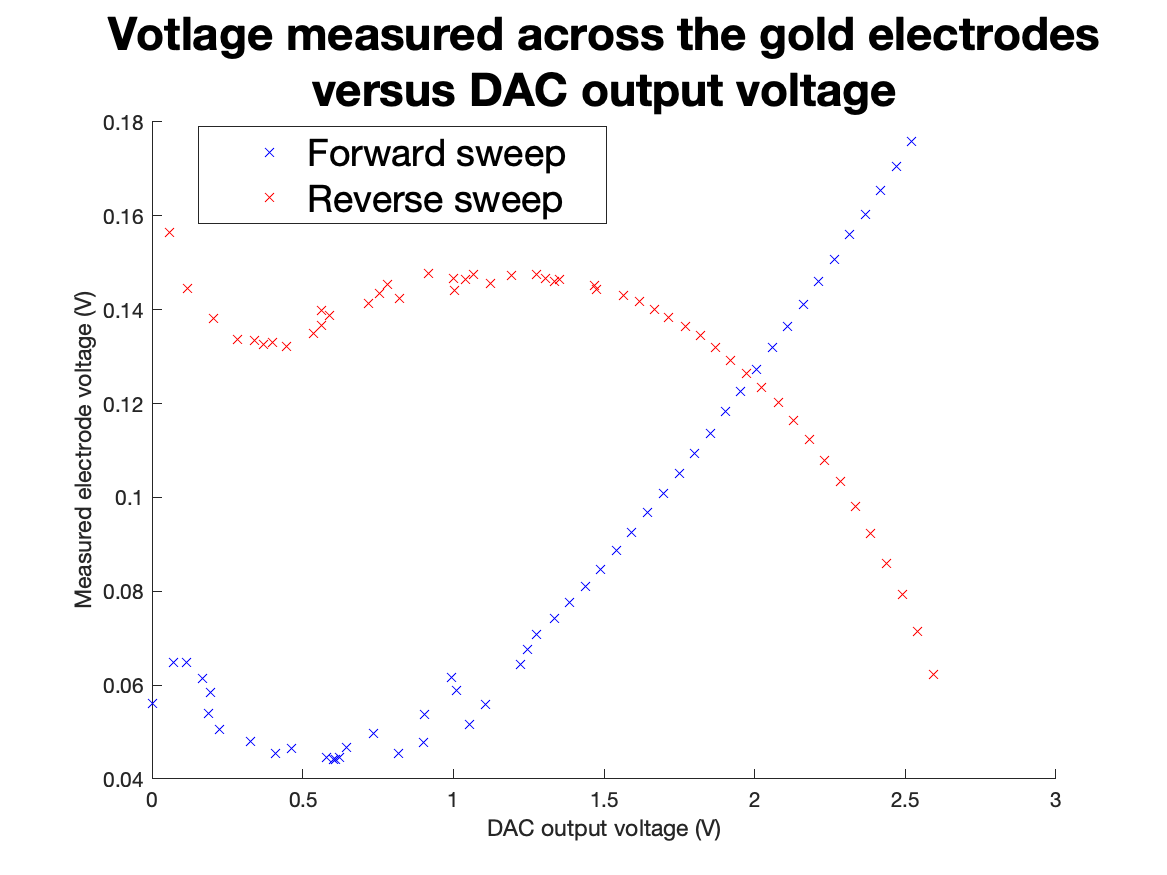
\includegraphics[width=\textwidth]{Figures/Testing/Aus2}
        \caption{Conductivity test 1 with gold electrodes and the fringe shield, a voltage range of $0-2,6V$, and 50 samples taken of salt water sample of unknown salinity.}
        \label{fig:test1} %chktex 24
    \end{minipage}
    \begin{minipage}{0.5\textwidth}
        \centering
        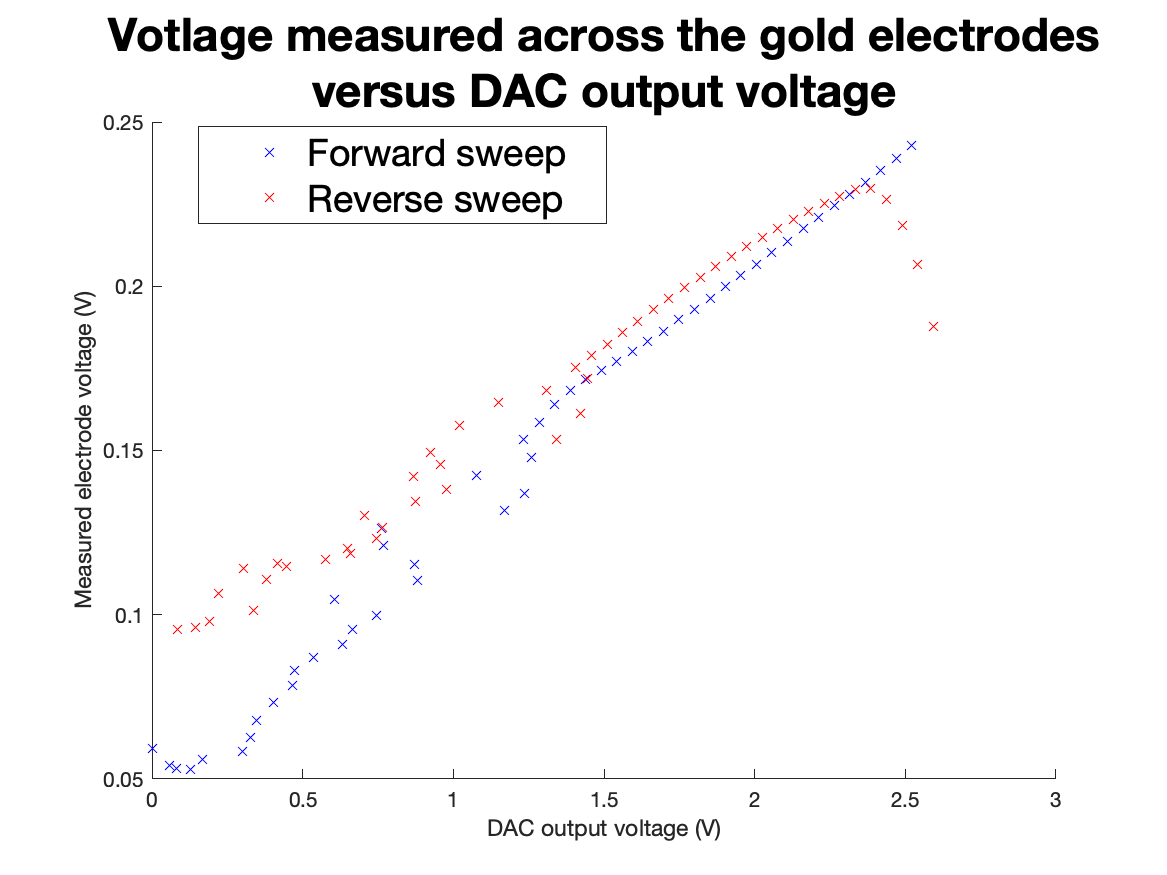
\includegraphics[width=\textwidth]{Figures/Testing/Aus3}
        \caption{Conductivity test 2 with draining and resetting the \gls{dac} between each voltage sample.}
        \label{fig:test2} %chktex 24
    \end{minipage}
\end{figure}

To further investigate the inconsistency, the \gls{dac} was drained and reset to $0V$ between each voltage sample before it was set to the desired voltage.
It should be noted that the \gls{dac} drain added a slight delay between each voltage sample of around $10ms$. 
While this did make the forward and reverse sweeps more similar, as shown in \reffig{fig:test2}, the initial voltage lag of the reverse sweep, at the higher voltages, was still present.

An alternative theory proposed that the measurements of the water briefly altered its properties, which in turn altered the proceeding measurements.
This alteration was unlikely to be a capacitive effect as the measurements were taken bidirectionally, which would have dissipated any built-up charge.
It was likely the voltage was dissociating the dissolved material into ions, allowing the charges in the salt water sample to move more freely~\cite{ostdiek_inquiry_into_physics_2020}.
However, determining exactly what was causing the alteration was beyond the scope of this project.

Instead, the theory was tested by taking priming measurements at the maximum voltage of $2,6V$ before capturing the actual measurements.
The priming caused the actual measurements in both directions to start high and progressively move to their predicted paths, as shown in \reffig{fig:test3}.

\begin{figure}[ht]
    \begin{minipage}{0.5\textwidth}
        \centering
        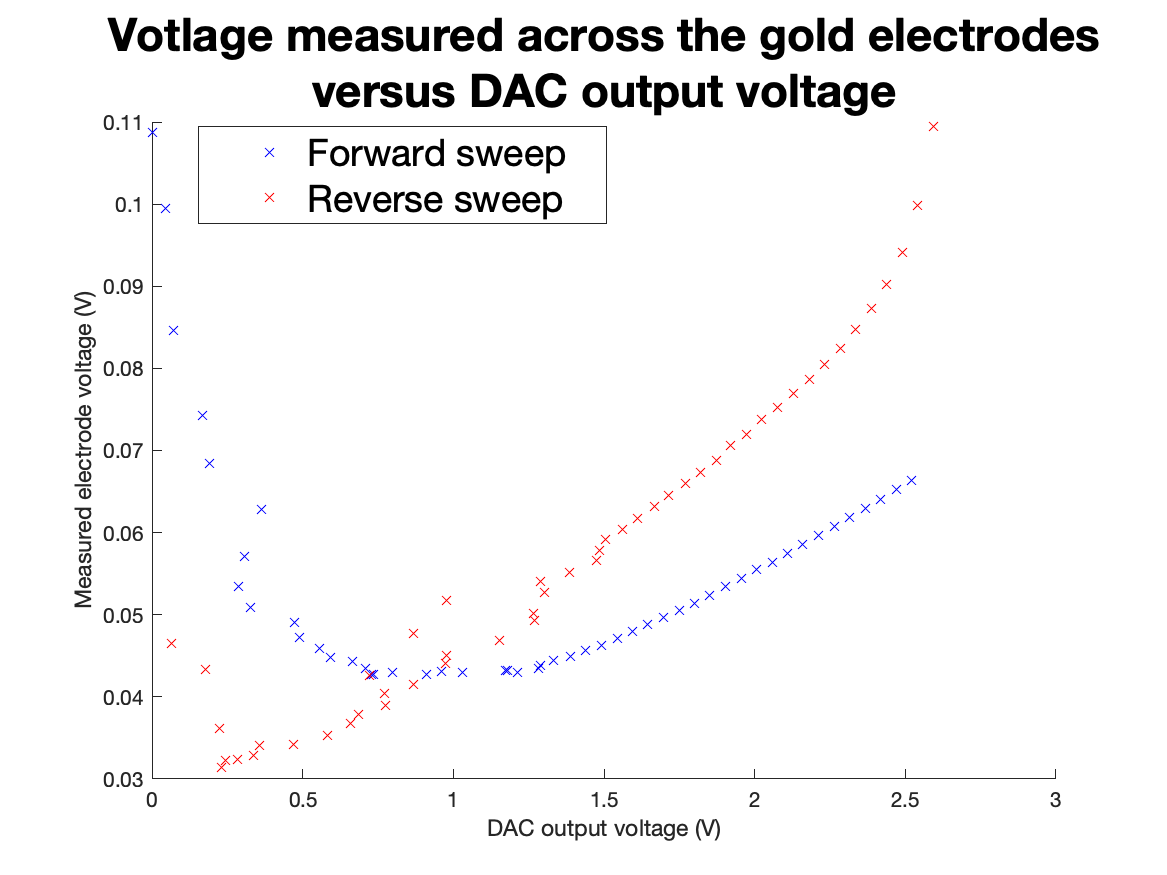
\includegraphics[width=\textwidth]{Figures/Testing/Aus5}
        \caption{Conductivity test 3 with 25 priming measurements taken before the actual measurement.}
        \label{fig:test3} %chktex 24
    \end{minipage}
    \begin{minipage}{0.5\textwidth}
        \centering
        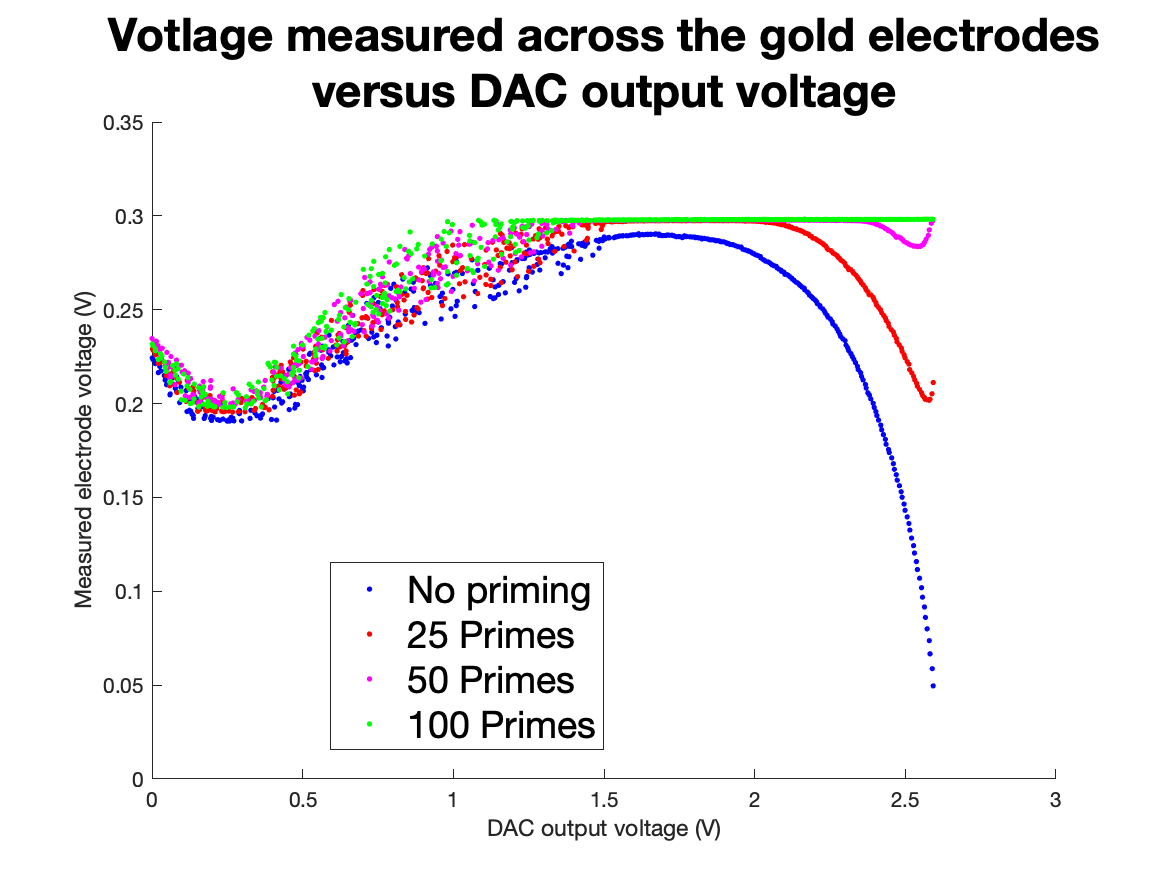
\includegraphics[width=\textwidth]{Figures/Testing/Aus7}
        \caption{Conductivity test 4 with a varying number of priming measurements and all true measurement taken as reverse voltage sweeps with 500 voltage samples.}
        \label{fig:test4} %chktex 24
    \end{minipage}
\end{figure}

This result supported the theory that the measurements were affecting the water.
The next test varied the number of priming measurements and used 500 voltage samples to increase the curve's resolution, as shown in \reffig{fig:test4}.
It should be noted that the voltage measurement effectively clipped at $0,3V$ as the output of the $11\times$ gain op-amp reached $0,3\times 11 = 3,3V$, which is the maximum voltage it can output.

While it was theoretically possible to perfectly prime a measurement, it was considered impractical, and it was also unlikely that the priming would have zero impact on the actual measurements.
Thus, voltage priming was not considered a viable solution for making repeatable measurements.
These results also indicated that a voltage measurement could be vulnerable to the priming effect from the previous measurement, which would cause undesirable effects.
Thus, an alternative method was needed to take the measurements.

The priming effect decreased over time, allowing the voltage sweeps in \reffig{fig:test3} to return to their expected curves.
A new theory stemmed from this that the water could relax from a primed state over time.
To test this, a delay, or relaxation time, was added between voltage samples, during which no voltage was applied to the electrodes.
The first test used a relaxation time of $2s$ and $500ms$.
With a $2s$ relaxation time, the forward and reverse voltage sweeps were near identical, as shown in \reffig{fig:test5}
However, with a $500ms$ relaxation time, there was a clear difference and the same initial voltage lag shown in \reffig{fig:test2}.

\begin{figure}[ht]
    \begin{minipage}{0.5\textwidth}
        \centering
        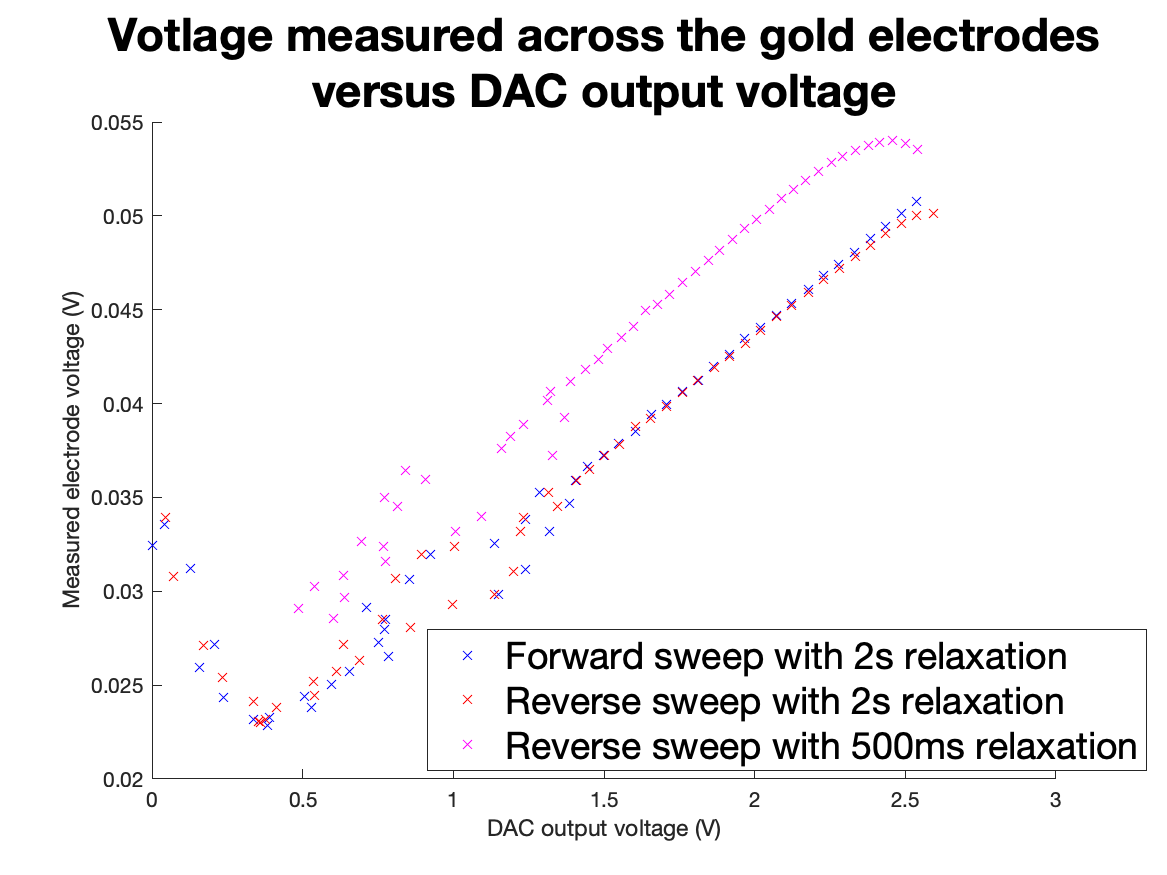
\includegraphics[width=\textwidth]{Figures/Testing/Aus8}
        \caption{Conductivity test 5 with a varying amount of relaxation time before each measurement was taken and 50 samples.}
        \label{fig:test5} %chktex 24
        \end{minipage}
    \begin{minipage}{0.5\textwidth}
        \centering
        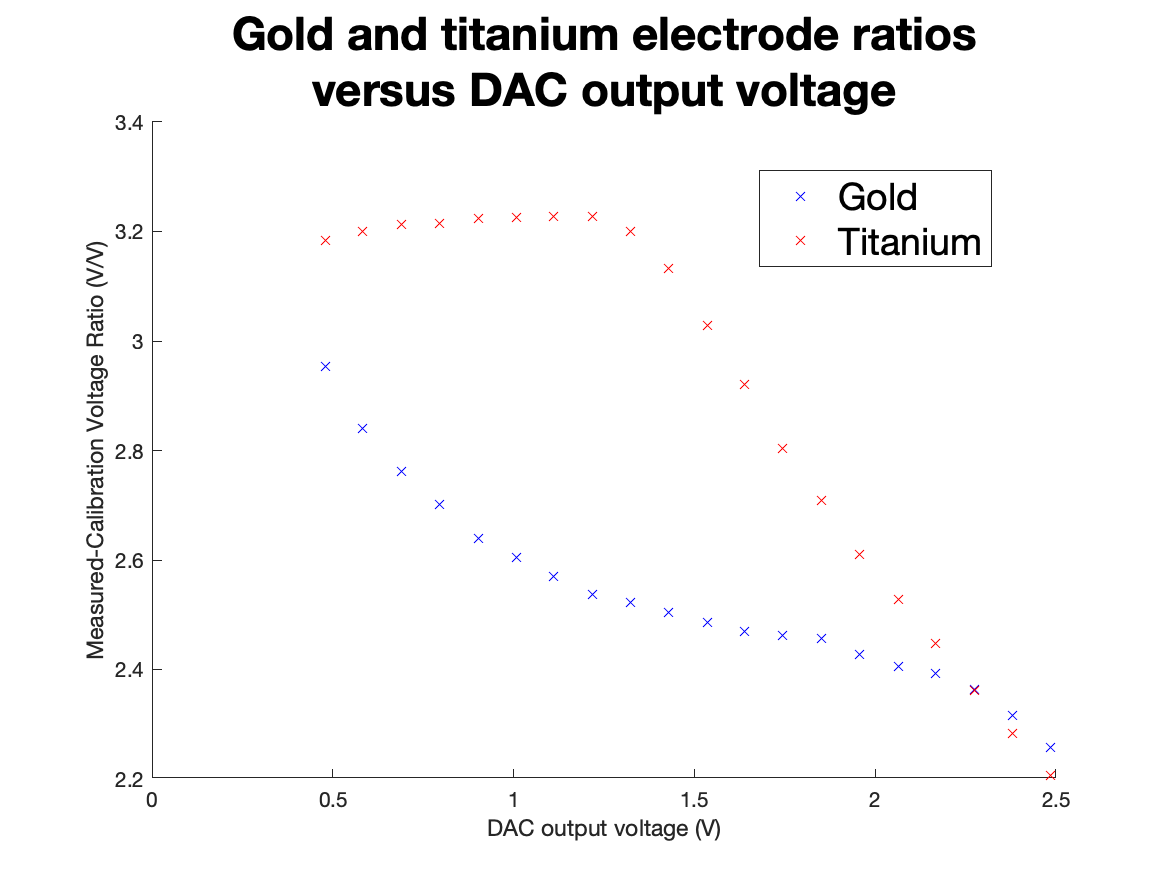
\includegraphics[width=\textwidth]{Figures/Testing/AusTi15}
        \caption{Conductivity test 6 with the difference between the titanium and gold electrodes.}
        \label{fig:test6} %chktex 24
    \end{minipage}
\end{figure}

This concluded a valid method of measuring a voltage sweep, which used a relaxation time of $2s$ between each voltage sample.
This allowed the titanium electrodes to be configured.
Iterative testing revealed that titanium electrodes $30m$ in length spaced $6mm$ apart provided a good balance with an $R_1$ value of $100\Omega$.
A test comparing the titanium and gold electrodes was performed, shown in \reffig{fig:test6}, which showed that the gold electrodes followed the expected curve that \refref{benjankar_ec_based_salt_measurement_2021} found, while the titanium electrodes did not.
The reason for this is unknown; it was theorised the fringing effect and conductivity of the titanium electrodes were the cause, which needed further investigation.



\begin{figure}[ht]
    \begin{minipage}{0.5\textwidth}
        \centering
        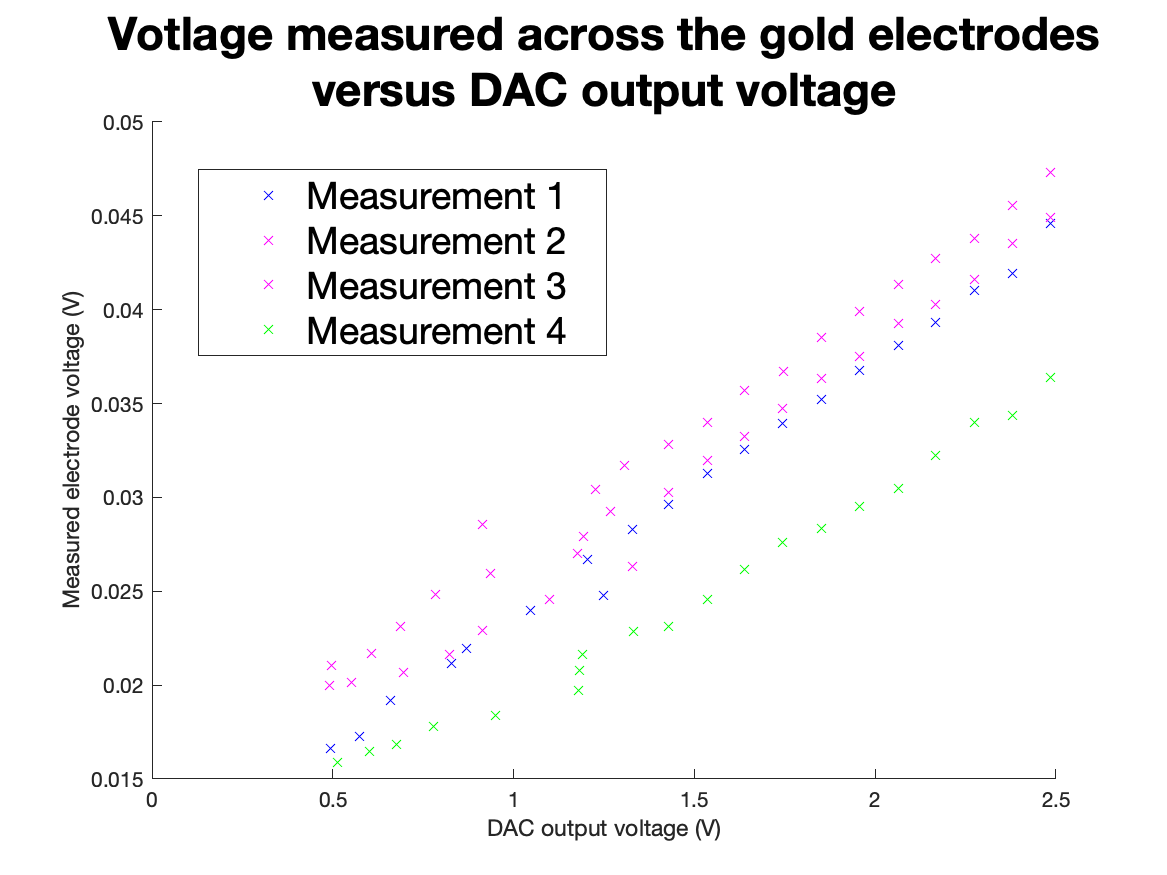
\includegraphics[width=\textwidth]{Figures/Testing/Aus12}
        \caption{Conductivity test 7 with 4 identical tests of 20 samples with 2s of relaxation time between measurements.}
        \label{fig:test7} %chktex 24
    \end{minipage}
    \begin{minipage}{0.5\textwidth}
        \centering
        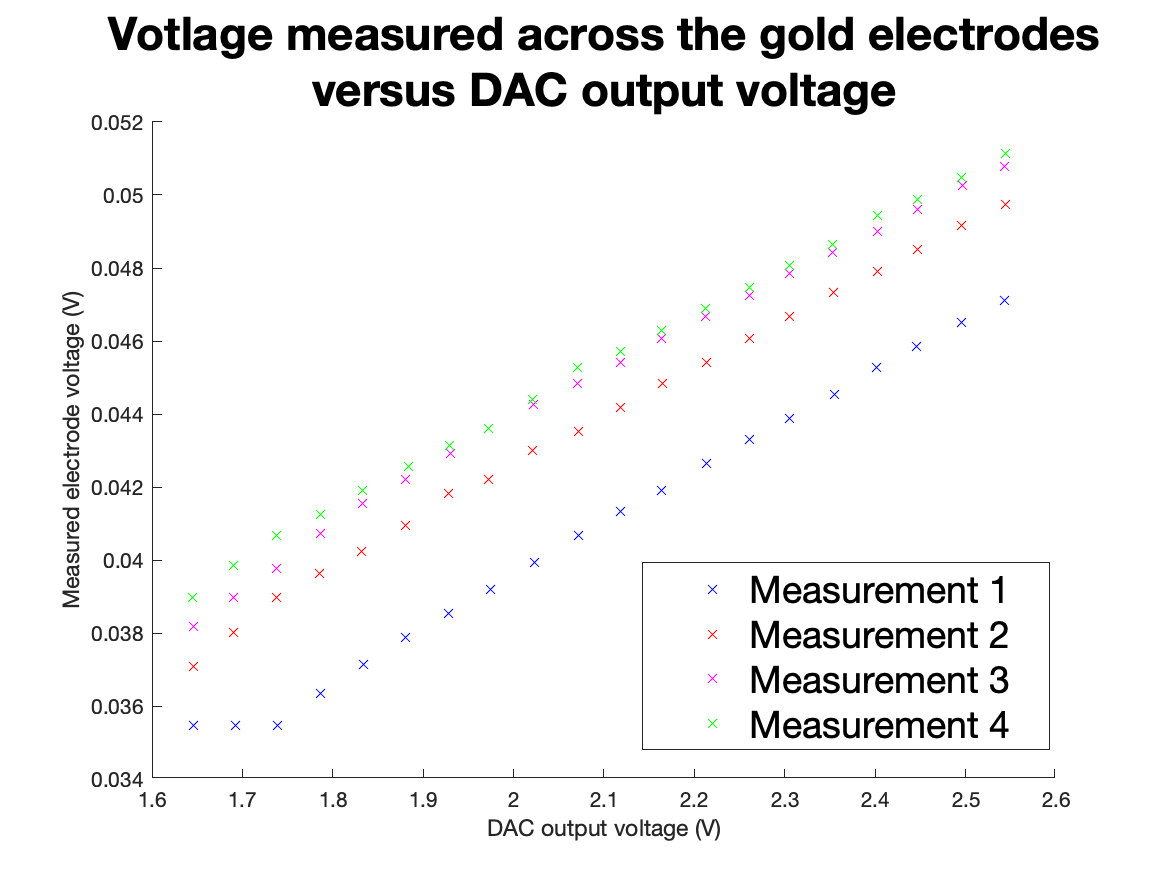
\includegraphics[width=\textwidth]{Figures/Testing/Aus10}
        \caption{Conductivity test 6 with 4 identical tests of 20 samples with 2s of relaxation time between measurements.}
        \label{fig:test8} %chktex 24
    \end{minipage}
\end{figure}

The last tests to conduct for the voltage sweep were to determine the repeatability of the measurements, and to determine if there was a measurable difference between two different salt water samples.
The first test took two samples of two different salt water samples with different salinities, the results of which can be seen in \reffig{fig:test7}.
This showed that the voltage sweeps were approximately grouped by salinity, and there was a clear difference between the two samples.
The next test aimed to prove repeatability of the measurement, taking 4 identical tests spaced shortly apart, shown in \reffig{fig:test8}.
The results showed that the measurements were approximately grouped.
However, it was noted that the sample's apparent conductivity was decreasing with each successive test, causing the measurements to drift upwards.

FIX.
The measurement inconsistency of the voltage samples below $1,5V$, shown in \reffig{fig:test5}, were present in both the electrode voltage measurement and calibration voltage measurement, and thus, were likely due to noise in either the \gls{adc} or op-amp.
It was decided to remove this voltage range, restricting the \gls{dac} to between $1,65V$ and $2,6V$, to make further data interpretation more straightforward.
Similarly, the inconsistency at the end of the voltage range, shown in \reffig{fig:test6}, was likely due to the voltage lag of the reverse sweep, and thus voltages above $2V$ were ignored.

\section{Voltage to Conductivity Mapping}\label{sec:voltage-conductivity-mapping}

The following tests aimed to investigate the relationship between the voltage and conductivity of a salt water sample.
This required samples of known salinity, which were created by mixing sea salt and distilled water, and a handheld conductivity meter to measure the samples which was accurate to $0,1$ on the Practical Salinity Scale PSS-78.

In order to correctly assess the relationship between the voltage and conductivity, the probe had to measure a standard solution of 35 on the Practical Salinity Scale PSS-78, which was at $15\degree C$ and $0dbar$.
To conduct this test, the $34,8$ salinity sample was placed in a fridge and cooled to below $15\degree C$.
It was then removed and 4 measurements were taken for each electrode type when the sample warmed to approximately $15\degree C$, shown in \reffig{fig:test9} and \reffig{fig:test10}.

\begin{figure}[ht]
    \begin{minipage}{0.5\textwidth}
        \centering
        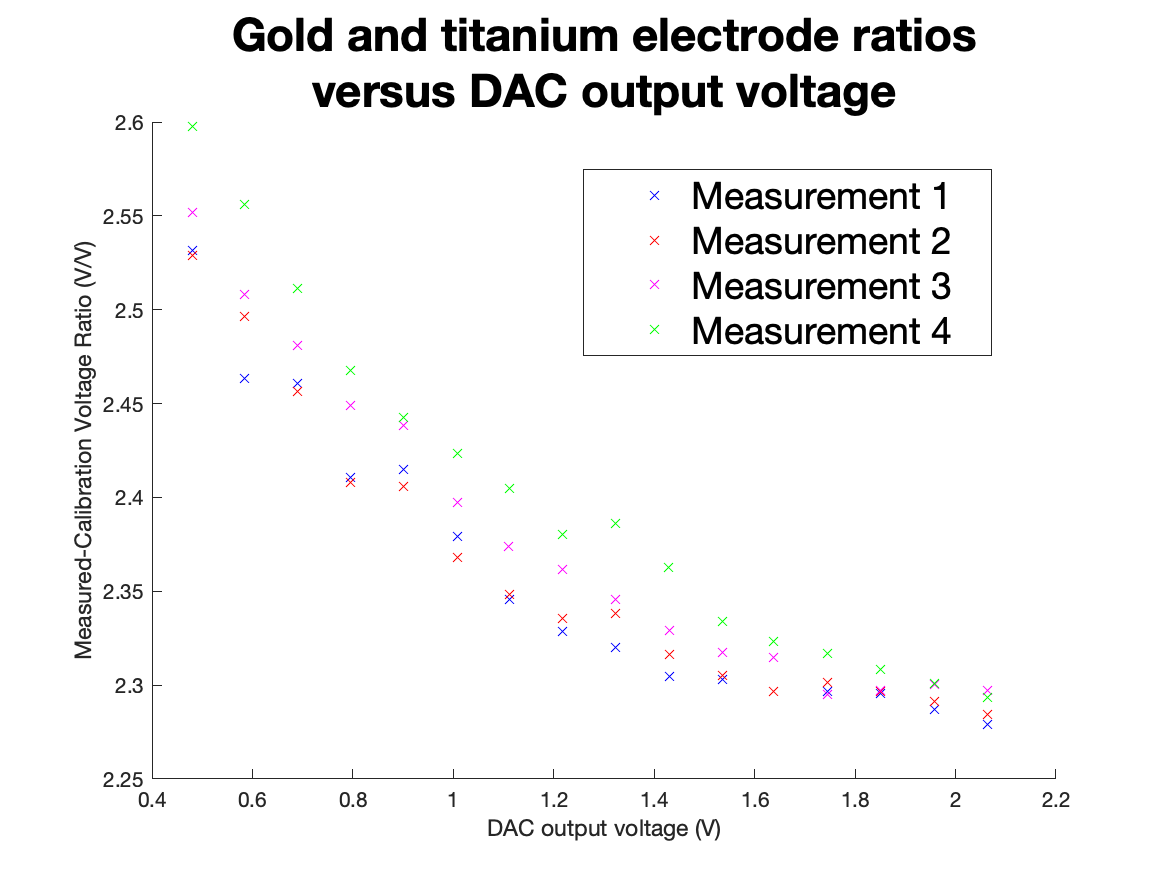
\includegraphics[width=\textwidth]{Figures/Testing/Aus16}
        \caption{Conductivity test 6 with 4 identical tests of 20 samples with 2s of relaxation time between measurements.}
        \label{fig:test9} %chktex 24
    \end{minipage}
    \begin{minipage}{0.5\textwidth}
        \centering
        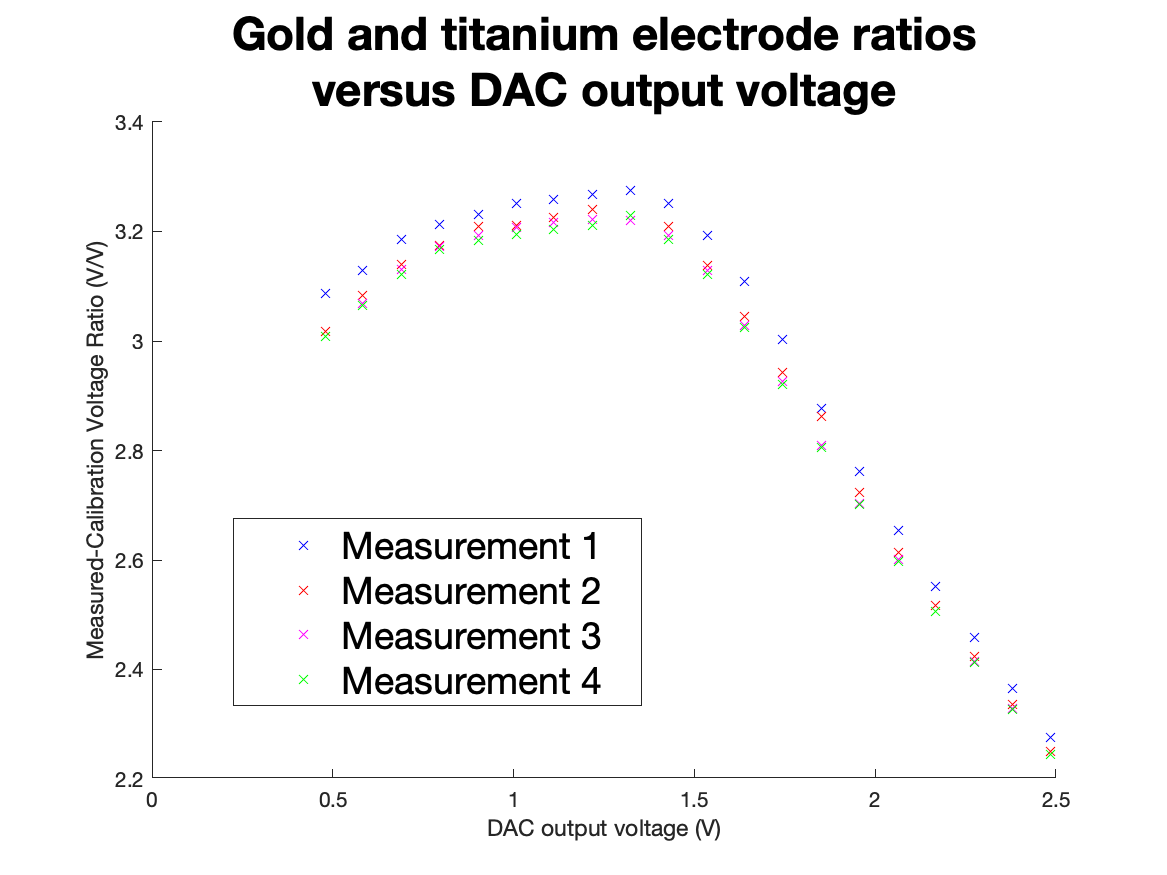
\includegraphics[width=\textwidth]{Figures/Testing/Ti16}
        \caption{Conductivity test 7 with 4 identical tests of 20 samples with 2s of relaxation time between measurements.}
        \label{fig:test10} %chktex 24
    \end{minipage}
\end{figure}

The gold electrode test showed a similar discovery to the voltage sweep tests, where the measurements were grouped but increased with each successive test.
The titanium electrode test showed a very different graph to the gold electrode test, appearing to have two different relationships present.
The samples taken below $1.4V$ appeared to be concave while the samples above $1.4V$ appeared to be convex, following a similar curve shape to the gold electrode test.
This was not due to the voltage clipping.
This was theorised to be due to the fringing effect of the titanium electrodes, which was overlaying with the resistance-voltage curve of the salt water sample.

The next tests examined salt water samples of different salinities with the goal of determining if the probe could calculate the salinity from the voltage measurements.
The samples were not measured at $15\degree C$, and thus their temperature was recorded and corrected for in the calculations.
The results of the $24,4$ \gls{psu} sample and the $29,1$ \gls{psu} sample for the gold and titanium electrodes are shown in \reffig{fig:test11} to \reffig{fig:test14}.

\begin{figure}[ht]
    \begin{minipage}{0.5\textwidth}
        \centering
        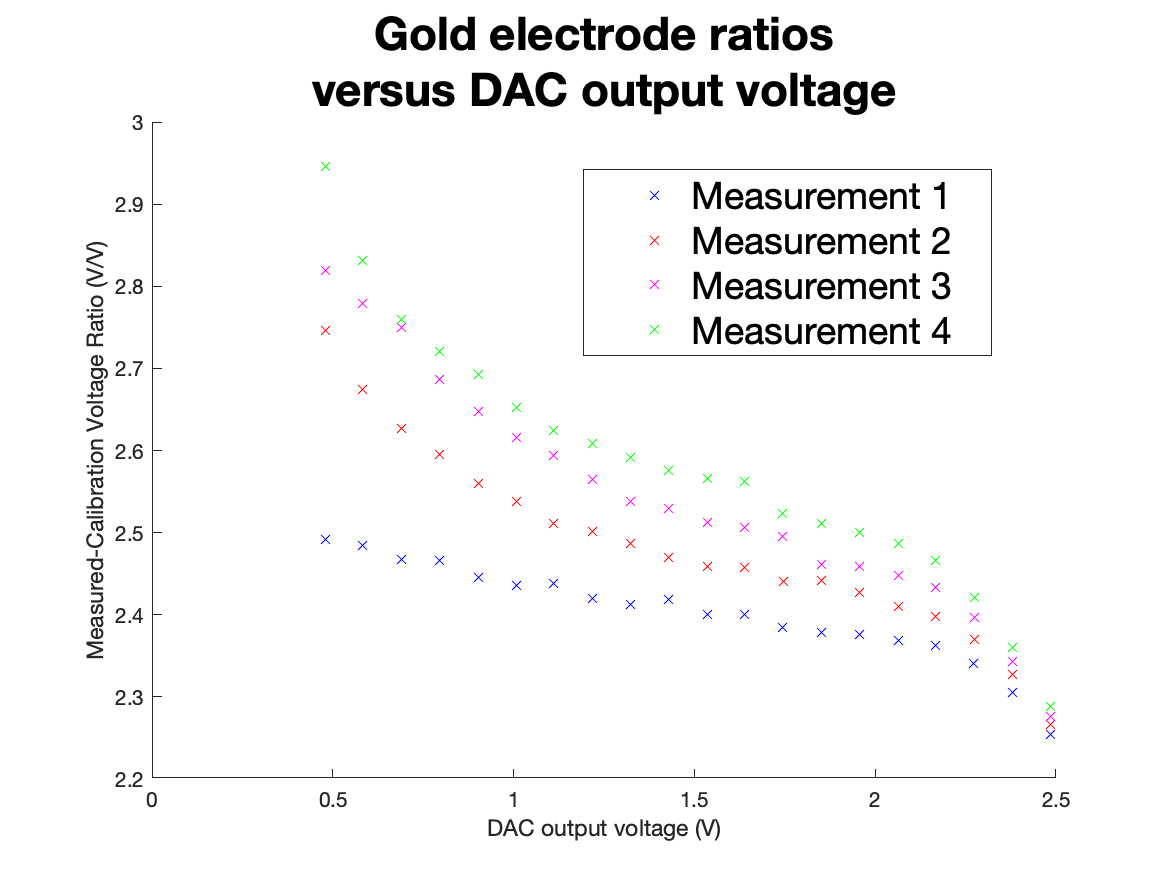
\includegraphics[width=\textwidth]{Figures/Testing/Aus17}
        \caption{Conductivity test 6 with 4 identical tests of 20 samples with 2s of relaxation time between measurements.}
        \label{fig:test11} %chktex 24
    \end{minipage}
    \begin{minipage}{0.5\textwidth}
        \centering
        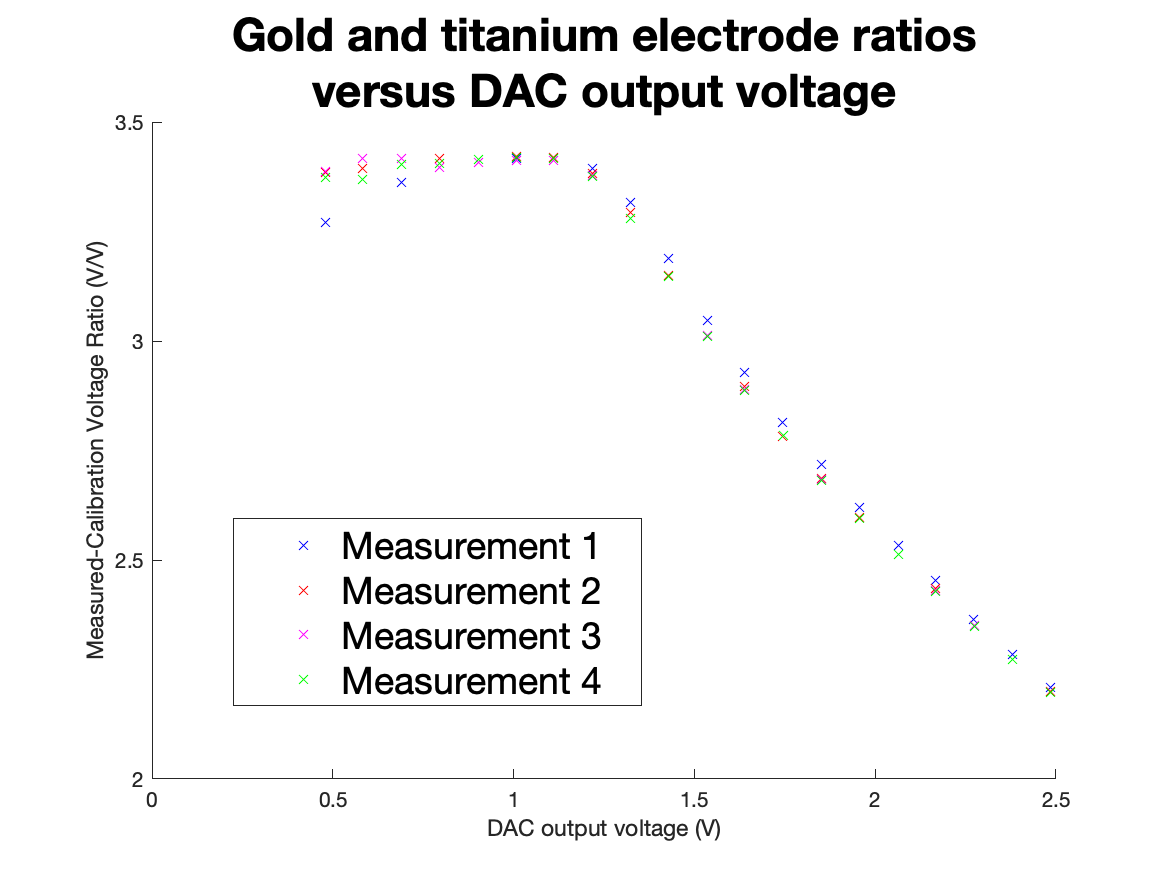
\includegraphics[width=\textwidth]{Figures/Testing/Ti17}
        \caption{Conductivity test 7 with 4 identical tests of 20 samples with 2s of relaxation time between measurements.}
        \label{fig:test12} %chktex 24
    \end{minipage}
\end{figure}

\begin{figure}[ht]
    \begin{minipage}{0.5\textwidth}
        \centering
        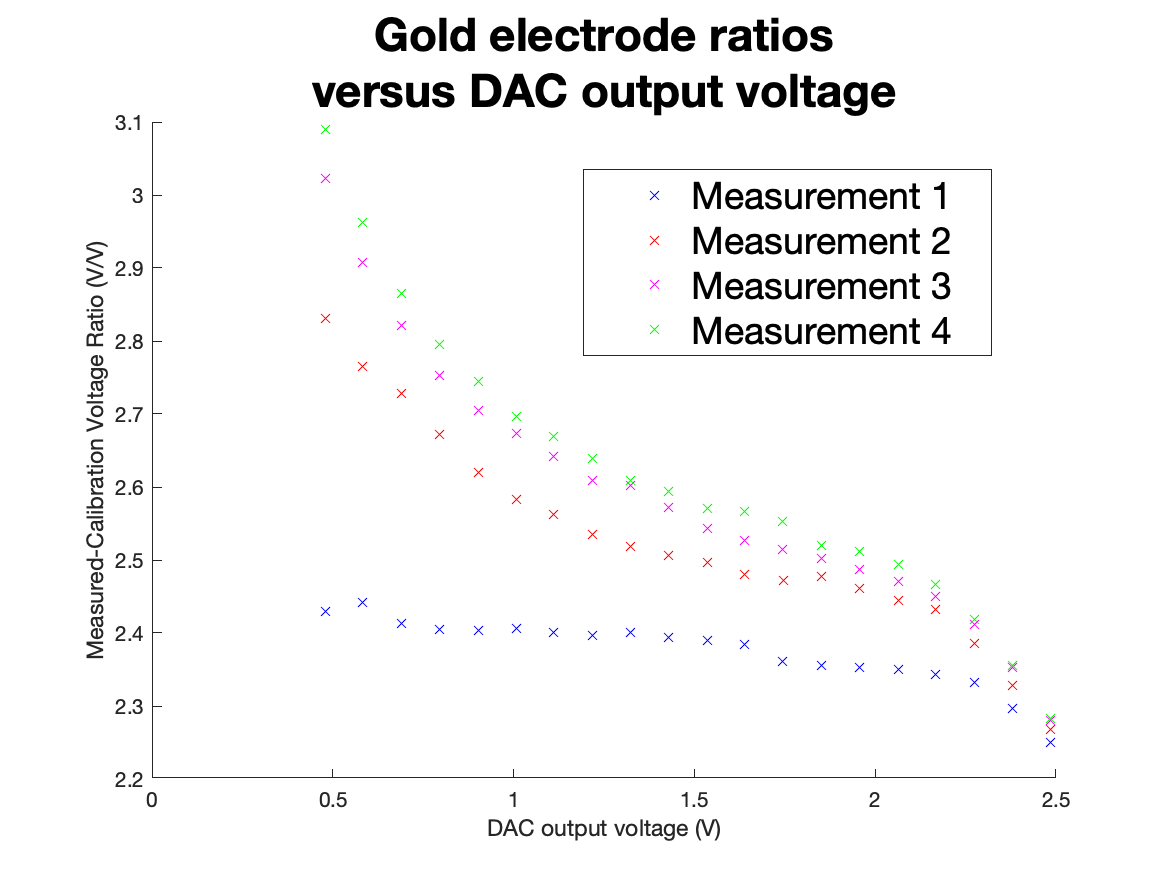
\includegraphics[width=\textwidth]{Figures/Testing/Aus18}
        \caption{Conductivity test 6 with 4 identical tests of 20 samples with 2s of relaxation time between measurements.}
        \label{fig:test13} %chktex 24
    \end{minipage}
    \begin{minipage}{0.5\textwidth}
        \centering
        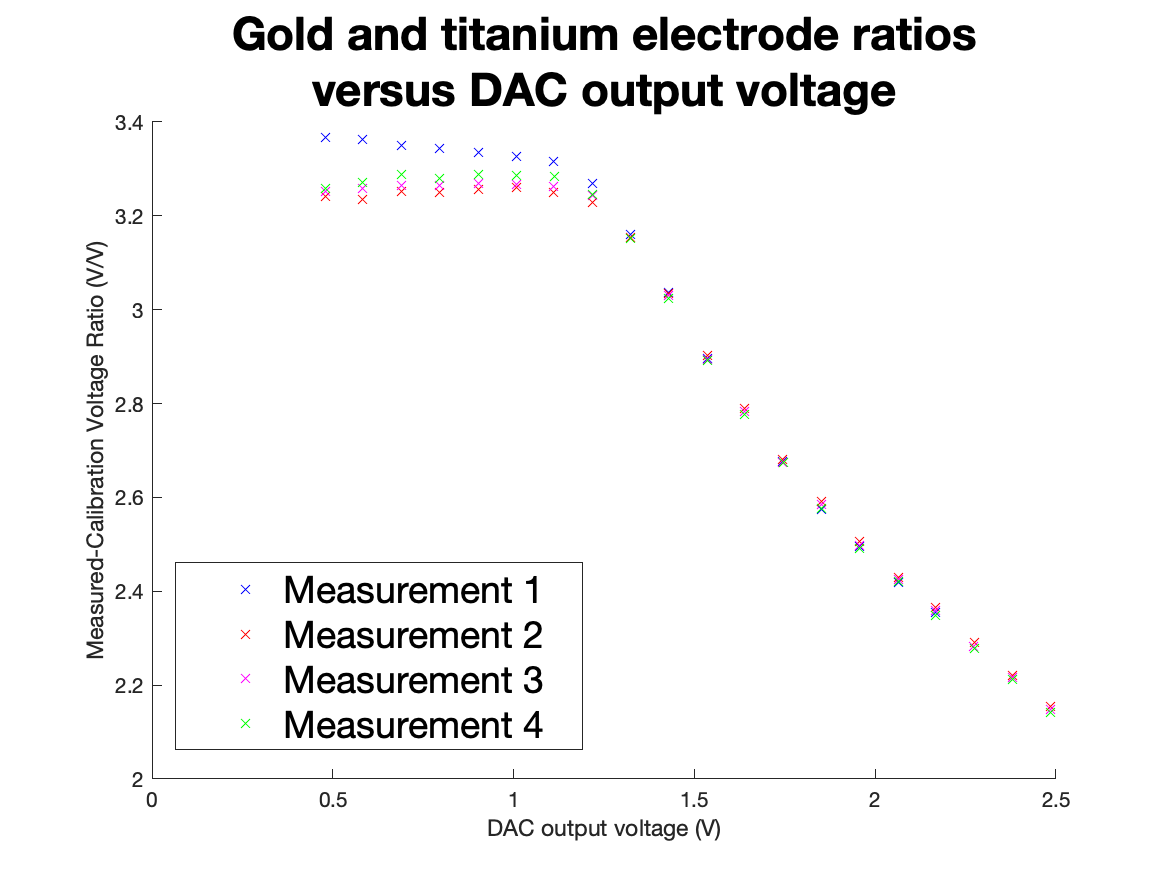
\includegraphics[width=\textwidth]{Figures/Testing/Ti18}
        \caption{Conductivity test 7 with 4 identical tests of 20 samples with 2s of relaxation time between measurements.}
        \label{fig:test14} %chktex 24
    \end{minipage}
\end{figure}

These results showed a similar trend to the tests performed on the standard solution, where the measurements were grouped but increased with each successive test.
The gold electrodes showed a similar trendline to the standard solution, while the titanium electrode's trendline was different below $1,4V$ and approximately the same above $1,4V$.

\begin{figure}[ht]
    \begin{minipage}{0.5\textwidth}
        \centering
        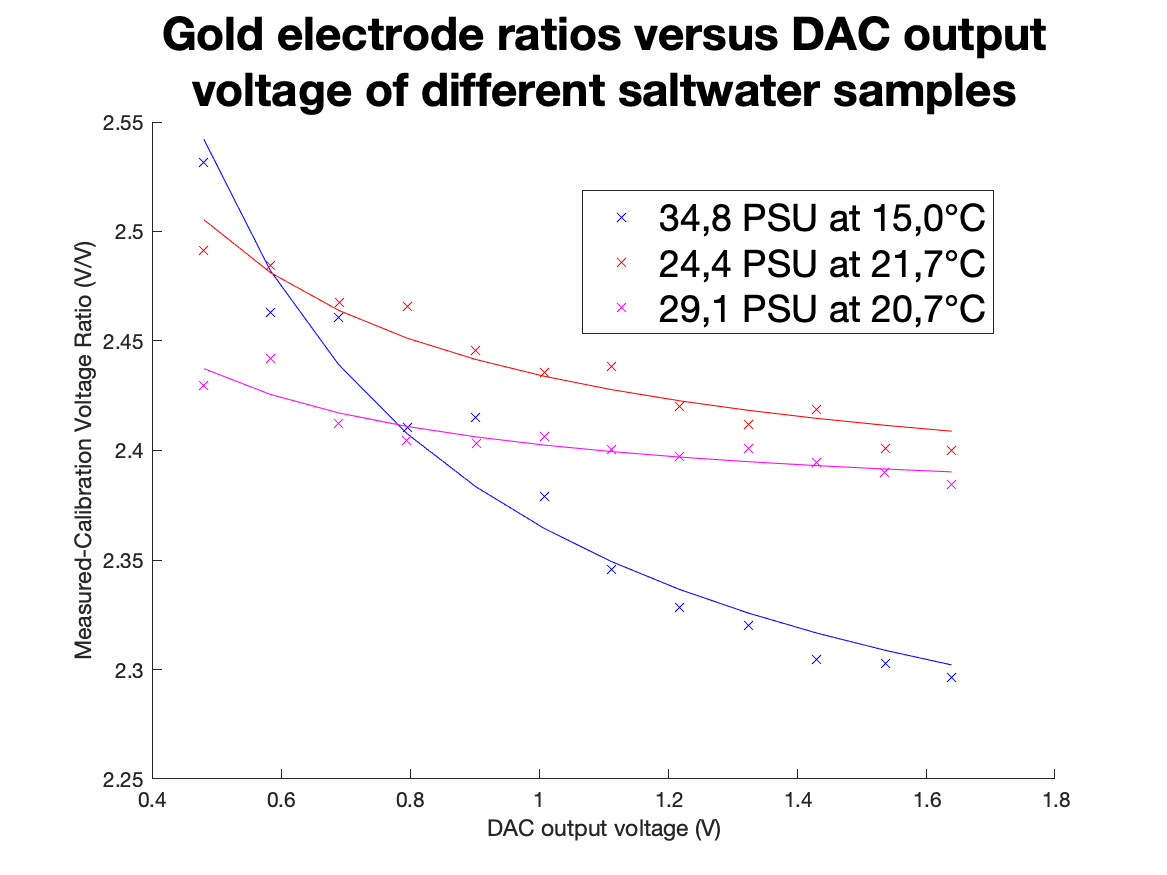
\includegraphics[width=\textwidth]{Figures/Testing/Au_sweep_analysis}
        \caption{Conductivity test 6 with 4 identical tests of 20 samples with 2s of relaxation time between measurements.}
        \label{fig:test15} %chktex 24
    \end{minipage}
    \begin{minipage}{0.5\textwidth}
        \centering
        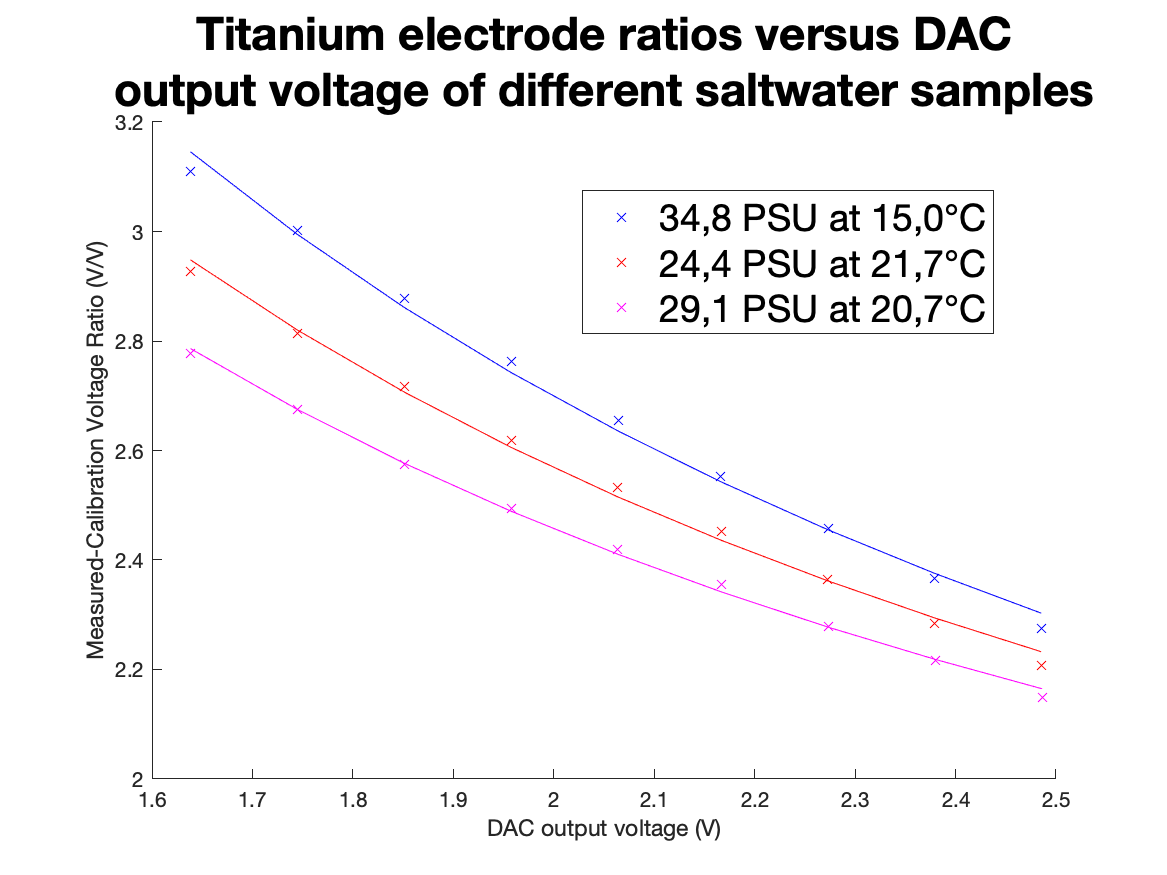
\includegraphics[width=\textwidth]{Figures/Testing/Ti_sweep_analysis}
        \caption{Conductivity test 7 with 4 identical tests of 20 samples with 2s of relaxation time between measurements.}
        \label{fig:test16} %chktex 24
    \end{minipage}
\end{figure}

waiting 2s per measurement for 50 samples took very long and an alternate method was to change the water infront of the electrodes by agitating/stirring the water.
this gave repeatable results that also showed a difference between two different water samples. GRAPH
taking fewer samples over the more linear voltage range gave something that was approximately linear.

trying to find a decernable metric from these graphs by analysing A/(s+p) between two samples of arbitrary salinity. TABLE

try repeated single measurements.

ac testing not rigged up correctly. GRAPH